\paragraph{}
Nos últimos anos o \textit{OpenSource} esta tendo uma evolução crescente, após empresas como Microsoft, Google e Facebook, começarem a disponibilizar alguns de seus \textit{softwares} utilizados internamente para a comunidade de \textit{software} livre.
Utilizando o GitHub, um dos maiores hubs de código e \textit{networking} de desenvolvedores do mundo, essas empresas conseguem disponibilizar seu \textit{software} em repositórios, locais de hospedagem de código, regido por uma licença, onde é descrito o que é exigido, permitido e proibido com o \textit{software} em questão.

\paragraph{}
Ao pesquisar sobre licenças de \textit{software} livre é possível encontrar uma alta gama de variedades para os mais diversos fins, tudo depende do ponto em que o mantenedor do projeto quer chegar, seja ele, trabalhar em comunidade (MIT), estar preocupado com patentes (Apache) ou apenas compartilhar melhorias (GPLv2/v3) \cite{choosealicense}.
Partindo-se do ponto em que a escolha de uma licença pode influenciar na popularidade de um projeto, conclui-se que isso é apenas uma pequena porcentagem comparado com o todo, no caso de ter uma grande empresa por trás denota-se grande possibilidade de o projeto ser bom e confiável, visto que, uma vez em que todos os desenvolvedores tem um acesso ao código e a possibilidade de estudar-lo, torna-se fácil a verificação de veracidade do projeto.

\paragraph{}
De acordo com a pesquisa de Borges \cite{borges2016understanding}, ele demonstra alguns \textit{insight's} para poder entender a popularidade de um determinado projeto. Inspirados pelos botões de redes sociais modernas, os usuários do GitHub também podem estrelar um repositório, presumivelmente para manifestar interesse ou satisfação com o projeto hospedado\cite{gousios2014exploratory, gousios2015work}.
Por exemplo, os desenvolvedores podem separar sua própria cópia de um repositório (\textit{Fork}), trabalhar e melhorar o código localmente e, em seguida, enviar uma solicitação para integrar as mudanças no repositório principal (\textit{Pull Request})\cite{borges2016understanding}. Gerando assim uma popularidade de alguns projetos, e tirando esse proveito de semelhanças com redes sociais fica mais fácil poder analisar o que é tendencia ou não, através de índices como demonstrado na Figura \ref{fig:github-linux}
\begin{figure}[ht!]
    \centering
    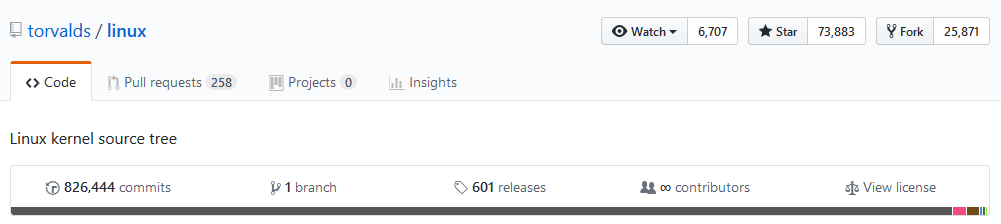
\includegraphics[width=\linewidth]{assets/images/github-linux.PNG}
    \caption{Exemplo de Índices no Github (Bootstrap)}
    \label{fig:github-linux}
\end{figure}

\paragraph{}
Este artigo tem como objetivo estudar a rede de desenvolvedores GitHub, mais especificamente os repositórios de software, analisando os \textit{insight's} comentados e utilizando metodos da matemática moderna para poder encontrar um padrão para cada determinado tipo de licença de software livre.